\Opensolutionfile{solution_file}[solutions/sols_010]
% в квадратных скобках фактическое имя файла

\chapter{МНК без матриц и вероятностей}

\begin{problem} %1.1
Пусть $a = (a_1,\dots,a_n)$ и $b = (b_1,\dots,b_n)$ — два произвольных вектора. Определите, какие равенства справедливы:
\begin{enumerate}
\item $\sum_{i=1}^n {(a_i-\bar a)} = 0$;
\item $\sum_{i=1}^n {(a_i-\bar a)^2} = \sum_{i=1}^n {(a_i-\bar a)a_i}$;
\item $\sum_{i=1}^n {(a_i-\bar a)(b_i-\bar b)} = \sum_{i=1}^n {(a_i-\bar a)b_i}$;
\item $\sum_{i=1}^n {(a_i-\bar a)(b_i-\bar b)} = \sum_{i=1}^n {a_i b_i}$;
\item $\sum_{i=1}^n a_i = n\bar a$;
\item $\sum_{i=1}^n (a_i - \bar a)^2 = \sum_{i=1}^n a_i^2 - n \bar a^2$;
\item $\sum_{i=1}^n a_i^2 = \left( \sum_{i=1}^n a_i \right)^2$;
\item $\sum_{i=1}^n a_i^2 = (n\bar a)^2$;
\item $\sum_{i=1}^n \bar a = n \bar a$;
\item $\sum_{i=1}^n a_i \bar a = n \bar a^2$;
\item $\sum_{i=1}^n {(a_i-\bar a)b_i} = 0$.
\end{enumerate}


\begin{sol}
\begin{enumerate}
\item Верно: \[\sum_{i=1}^{n}(a_i-\bar{a}) = \sum_{i=1}^{n}a_i - n\cdot\bar{a} = \sum_{i=1}^{n}a_i - \sum_{i=1}^{n}a_i = 0\]
\item Верно: \[\sum_{i=1}^{n}(a_i-\bar{a})^2 = \sum_{i=1}^{n}(a_i-\bar{a})(a_i+\bar{a}) = \sum_{i=1}^{n}(a_i-\bar{a})a_i + \bar{a}\underbrace{\sum_{i=1}^{n}(a_i-\bar{a})}_{=0} = \sum_{i=1}^{n}(a_i-\bar{a})a_i \]

\item Верно: \[\sum_{i=1}^{n}(a_i-\bar{a})(b_i-\bar{b}) = \sum_{i=1}^{n}(a_i-\bar{a})b_i - \bar{b}\underbrace{\sum_{i=1}^{n}(a_i-\bar{a})}_{=0} = \sum_{i=1}^{n}(a_i-\bar{a})b_i \]
\item А вот это неверно! (следует из предыдущего пункта)
\item Верно
\item Верно
\item Неверно
\item Неверно
\item Верно
\item Верно: \[\sum_{i=1}^{n}a_i\bar{a} = \frac{n}{n}\bar{a}\sum_{i=1}^{n}a_i = n \bar{a} \frac{\sum_{i=1}^{n}a_i}{n} = n\bar{a}^2 \]
\item Неверно (см. пунк 3)
\end{enumerate}
\end{sol}
\end{problem}





\begin{problem} %1.2
При помощи метода наименьших квадратов найдите оценку неизвестного параметра $\theta$ в следующих моделях:

\begin{enumerate}
\item $y_i = \theta + \theta x_i + \varepsilon_i$;
\item $y_i = \theta - \theta x_i + \e_i$;
\item $\ln y_i = \theta + \ln x_i + \e_i$;
\item $y_i = \theta + x_i + \e_i$;
\item $y_i = 1 + \theta x_i + \e_i$;
\item $y_i = \theta / x_i + \e_i$;
\item $y_i = \theta x_i + (1-\theta)z_i+\e_i$.
\end{enumerate}


\begin{sol}
\begin{enumerate}
\item \(\htheta = \sum y_i (1 + x_i) / \sum (1 + x_i)^2\)

Стандартная процедура МНК:
\[RSS = \sum \e_i^2 = \sum \left(y_i - \theta - \theta x_i\right)^2 \rightarrow \min \limits_\theta\]
\[\frac{\partial RSS}{\partial \theta} = 2 \sum \left(y_i - \theta - \theta x_i\right)(-1 - x_i) \]
\[\sum \left(y_i - \htheta - \htheta x_i\right)(-1 - x_i) = 0\]
\[\sum y_i (-1 - x_i) + \htheta \sum (-1 - x_i)^2 = 0 \]
\[\htheta = \frac{\sum y_i (1 + x_i)}{\sum (1 + x_i)^2} \]

\item \(\htheta = \sum \left(y_i (1 - x_i)\right) / \sum (1 - x_i)^2\)

\item \(\htheta = \left( \sum \text{ln} (y_i / x_i) \right) / n \)

\item \(\htheta = \left( \sum (y_i - x_i) \right) / n \)

\item \(\htheta = \sum \left((y_i - 1) x_i\right) / \sum x_i^2\)

\item \(\htheta = \sum (y_i / x_i^2) / \sum (1 /x^3)\)

\item \(\htheta = \sum \left((y_i - z_i)(x_i - z_i) \right) / \sum \left(x_i - z_i\right)^2 \)

\end{enumerate}
\end{sol}
\end{problem}


\begin{problem} %1.3
Покажите, что для моделей $y_i= \alpha + \beta x_i + \e_i$, $z_i = \gamma + \delta x_i + \upsilon_i$ и $y_i + z_i = \mu + \lambda x_i + \xi_i$ МНК-оценки связаны соотношениями $\hat{\mu}=\hat{\alpha}+\hat{\gamma}$ и $\hat{\lambda}=\hb + \hat{\delta}$.


\begin{sol}
Заметим, что $y_i + z_i = \underbrace{(\alpha + \gamma)}_{\mu} + \underbrace{(\beta+\delta)}_{\lambda}x_i + u_i$.

Если оценить данную модель при помощи МНК, получим как раз то, что нужно доказать.
\end{sol}
\end{problem}


\begin{problem} %1.4
Найдите МНК-оценки параметров $\alpha$ и $\beta$ в модели $y_i = \alpha + \beta y_i + \e_i$.


\begin{sol}
\(\hat{\alpha} = 0, \ \hb = 1 \)
\end{sol}
\end{problem}


\begin{problem} %1.5
Рассмотрите модели $y_i = \alpha + \beta (y_i + z_i) + \e_i$, $z_i = \gamma + \delta(y_i+z_i) + \e_i$.
\begin{enumerate}
\item Как связаны между собой $\hat{\alpha}$ и $\hat{\gamma}$?
\item Как связаны между собой $\hb$ и $\hat{\delta}$?
\end{enumerate}


\begin{sol} % 1.5.
Рассмотрим регрессию суммы $(y_i + z_i)$ на саму себя. Естественно, в ней
\[
\widehat{y_i + z_i} = 0 + 1 \cdot (y_i + z_i).
\]

Отсюда получаем, что $\hat{\alpha} + \hat{\gamma} = 0$ и $\hb + \hat{\delta} = 1$.
\end{sol}
\end{problem}




\begin{problem} %1.6
Как связаны МНК-оценки параметров $\alpha, \beta$ и $\gamma, \delta$ в моделях $y_i = \alpha + \beta x_i + \e_i$ и $z_i = \gamma + \delta x_i + \upsilon_i$, если $z_i = 2 y_i$?


\begin{sol}

Исходя из условия, нужно оценить методом МНК коэффициенты двух следующих моделей:
\[y_i = \alpha + \beta x_i + \e_i \]
\[y_i = \frac{\gamma}{2} + \frac{\delta}{2} x_i + \frac{1}{2} v_i \]

Заметим, что на минимизацию суммы квадратов остатков коэффициент \(1/2\) не влияет, следовательно:
\[\hat{\gamma} = 2\hat{\alpha}, \ \hat{\delta} = 2 \hb  \]

\end{sol}
\end{problem}


\begin{problem} %1.6
Для модели $y_i = \beta_1 x_i + \beta_2 z_i + \e_i$ решите условную задачу о наименьших квадратах:
\[
Q(\beta_1, \beta_2) := \sum_{i=1}^n (y_i - \beta_1 x_i - \beta_2 z_i)^2 \rightarrow \underset{\beta_1 + \beta_2 = 1}{\min}.
\]


\begin{sol}
Выпишем задачу:
\[
\begin{cases}
RSS = \sum\limits_{i=1}^{n}(y_i - \beta_1x_i - \beta_2z_i)^2 \rightarrow \min\limits_{\beta_1, \beta_2}\\
\beta_1 + \beta_2 = 1
\end{cases}
\]

Можем превратить ее в задачу минимизации функции одного аргумента:
\[
RSS =  \sum\limits_{i=1}^{n}(y_i - x_i - \beta_2(z_i-x_i))^2 \rightarrow \min_{\beta_2}
\]

Выпишем условия первого порядка:
\[
\frac{\partial RSS}{\partial \beta_2} = \sum\limits_{i=1}^{n}2(y_i-x_i-\hb_2(z_i-x_i))(x_i-z_i)=0
\]

Отсюда:
\[
\sum\limits_{i=1}^{n}(y_i-x_i)(x_i-z_i) + \hb_2\sum\limits_{i=1}^{n}(z_i-x_i)^2 = 0 \Rightarrow \hb_2 = \frac{\sum\limits_{i=1}^n (y_i-x_i)(z_i-x_i)}{\sum\limits_{i=1}^n (z_i-x_i)^2}
\]

А оценка $\beta_1$ найдется из соотношения $\hb_1+\hb_2 = 1$.

\end{sol}
\end{problem}




\begin{problem} %1.8
Даны $n$ пар чисел: $(x_1, y_1)$, \ldots, $(x_n,y_n)$. Мы прогнозируем $y_i$ по формуле $\hy_i=\hb x_i$. Найдите $\hb$ методом наименьших квадратов.


\begin{sol}
$\hb=\sum x_i y_i/\sum x_i^2$
\end{sol}
\end{problem}


\begin{problem} %1.9
Даны $n$ чисел: $y_1$, \ldots, $y_n$. Мы прогнозируем $y_i$ по формуле $\hy_i=\hb$. Найдите $\hb$ методом наименьших квадратов.

\begin{sol}
Нужно решить задачу:
\[
RSS = \sum\limits_{i=1}^n(y_i-\beta)^2 \rightarrow \min\limits_{\beta}
\]

Условия первого порядка:
\[
\frac{\partial RSS}{\partial \beta} = \sum\limits_{i=1}^{n}2(y_i-\hb) = 0 \Rightarrow \sum\limits_{i=1}^n y_i-n\hb = 0
\]

Поэтому
\[
\hb = \frac{\sum_{i=1}^ny_i}{n} = \bar{y}
\]
\end{sol}
\end{problem}


\begin{problem} % 1.10
Даны $n$ пар чисел: $(x_1, y_1)$, \ldots, $(x_n,y_n)$. Мы прогнозируем $y_i$ по формуле $\hy_i=\hb_1+\hb_2 x_i$. Найдите $\hb_1$ и $\hb_2$ методом наименьших квадратов.

\begin{sol}
$\hb_2=\sum (x_i-\bar{x})(y_i-\bar{y})/\sum(x_i-\bar{x})^2$, $\hb_1=\bar{y}-\hb_2\bar{x}$
\end{sol}
\end{problem}


\begin{problem}%1.11
Даны $n$ пар чисел: $(x_1, y_1)$, \ldots, $(x_n,y_n)$. Мы прогнозируем $y_i$ по формуле $\hy_i=1+\hb x_i$. Найдите $\hb$ методом наименьших квадратов.

\begin{sol}
Имеем следующую задачу:
\[
RSS = \sum\limits_i(y_i-1-\beta x_i)^2 \rightarrow \min\limits_{\beta}
\]

Откуда сразу все находим:
\[
\frac{\partial RSS}{\partial \beta} = \sum\limits_i2(y_i-1-\hb x_i)(-x_i) = 0 \Rightarrow \sum\limits_i (y_i-1-\hb x_i)x_i=0 \Rightarrow
\]
\[
\sum\limits_i x_iy_i-\sum\limits_ix_i - \hb\sum\limits_ix_i^2 = 0 \Rightarrow \hb = \frac{\sum_ix_i(y_i-1)}{\sum_ix_i^2}
\]
\end{sol}
\end{problem}


\begin{problem} %1.12
Перед нами два золотых слитка и весы, производящие взвешивания с ошибками. Взвесив первый слиток, мы получили результат $300$ грамм, взвесив второй слиток — $200$ грамм, взвесив оба слитка — $400$ грамм. Оцените вес каждого слитка методом наименьших квадратов.

\begin{sol}
Обозначив вес первого слитка за \(\beta_1\), вес второго слитка за \(\beta_2\), а показания весов за \(y_i\), получим, что
\[y_1 = \beta_1 + \e_1, \ y_2 = \beta_2 + \e_2, \ y_3 = \beta_1 + \beta_2 + \e_3\]

Тогда
\[(300 - \beta_1)^2 + (200 - \beta_2)^2 + (400 - \beta_1 - \beta_2)^2 \rightarrow \min \limits_{\beta_1,\  \beta_2} \]
\[\hb_1 = \frac{800}{3}, \ \hb_2 = \frac{500}{3} \]
\end{sol}
\end{problem}



\begin{problem} %1.13
Аня и Настя утверждают, что лектор опоздал на 10 минут. Таня считает, что лектор опоздал на 3 минуты. С помощью МНК оцените, на сколько минут опоздал лектор.

\begin{sol}

Ане, Насте и Тане нужно оценить модель $y_i = \beta + \e_i$. Для этого они должны решить следующую задачу:

\[RSS = 2(10-\beta)^2 + (3-\beta)^2\rightarrow \min \limits_{\beta}\]

\[\frac{\partial RSS}{\partial \beta} = -4(10-\beta)-2(3-\beta) \]

Условия первого порядка:

\[-4(10-\hb)-2(3-\hb)=0\]

\[20 - 2\hb +3 -\hb=0\]

\[3\hb = 23\]

\[\hb = \frac{23}{3}\]

\end{sol}
\end{problem}



\begin{problem} %1.14
Функция $f(x)$ непрерывна на отрезке $[0;1]$. Найдите аналог МНК-оценок для регрессии без свободного члена в непрерывном случае. Более подробно: найдите минимум по $\hb$ для функции
\[
Q(\hb)= \int_0^1 (f(x)-\hb x)^2\,dx.
\]

\begin{sol}
Условие первого порядка $\int_0^1 -2x(f(x)-\hb x) \, dx =0$, получаем
\[
\hb = \frac{\int_0^1 x f(x)\, dx} {\int_0^1 x^2 \, dx}
\]

\(\hb = \left(\int \limits_0^1 f(x) x dx\right) / \left(\int \limits_0^1 x^2 dx\right)\)
\end{sol}
\end{problem}



\begin{problem} %1.15
Есть двести наблюдений. Вовочка оценил модель $\hy=\hb_1+\hb_2 x$ по первой сотне наблюдений. Петечка оценил модель $\hy=\hat{\gamma}_1+\hat{\gamma}_2 x$ по второй сотне наблюдений. Машенька оценила модель $\hy=\hat{m}_1+\hat{m}_2 x$ по всем наблюдениям.
\begin{enumerate}
\item Возможно ли, что $\hb_2>0$, $\hat{\gamma}_2>0$, но $\hat{m}_2<0$?
\item Возможно ли, что $\hb_1>0$, $\hat{\gamma}_1>0$, но $\hat{m}_1<0$?
\item Возможно ли одновременное выполнение всех упомянутых условий?
\end{enumerate}


\begin{sol}
\begin{enumerate}
\item Проявите воображение! Все зависит от данных. Например, может быть вот так:

\begin{minted}[mathescape,
               linenos,
               numbersep=5pt,
               frame=lines,
               framesep=2mm]{r}
tikz("../R_plots/aggregate_regression.tikz", standAlone = FALSE, bareBones = TRUE)
n <- 100;
s <- rep(c(0, 4), c(n/2, n/2));
x <- c(1 + runif(n/2), runif(n/2));
y <- 2 * x + s + rnorm(n, sd = 0.15)


plot(x, y, type = "n", frame = "FALSE")
points(x[1 : (n/2)], y[1 : (n/2)], pch = 21,
       col = "black", bg = "ForestGreen", cex = 2)
points(x[(n/2 + 1) : n], y[(n/2 + 1) : n],
       pch = 21, col = "black", bg = "SkyBlue", cex = 2)

modelV1 <- lm(y ~ x + s)
# модели по 1:100 и 101:200 в отдельности
abline(coef(modelV1)[1], coef(modelV1)[2], lwd = 3)
abline(coef(modelV1)[1] + 4 * coef(modelV1)[3],
       coef(modelV1)[2], lwd = 3)
modelV2 <- lm(y ~ x)
# общая модель
abline(modelV2, lwd = 2, col = "red")
invisible(dev.off())
\end{minted}

\begin{minipage}{0.6\textwidth}
\begin{center}
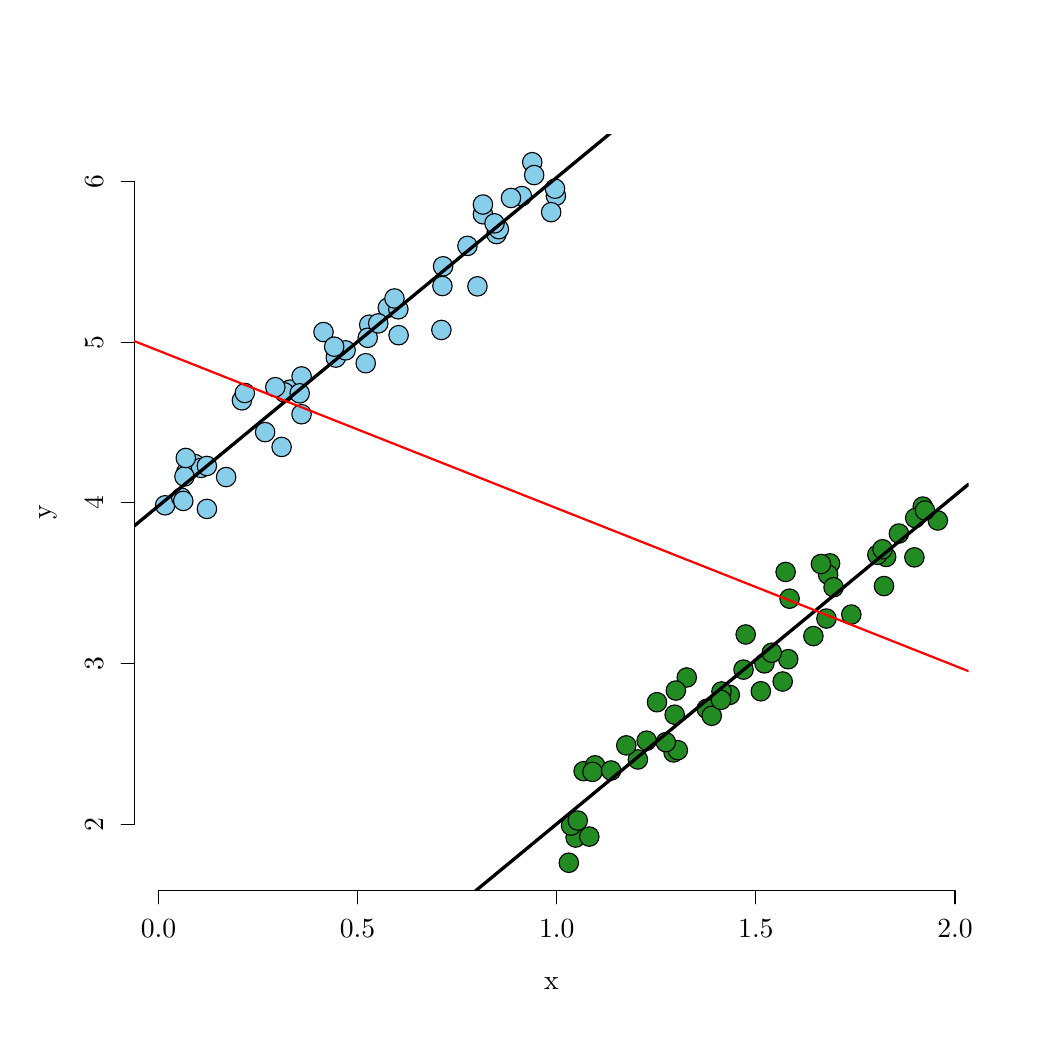
\begin{tikzpicture}[scale = 0.025]
% Created by tikzDevice version 0.10.1 on 2016-04-10 00:22:30
% !TEX encoding = UTF-8 Unicode
\definecolor{fillColor}{RGB}{255,255,255}
\path[use as bounding box,fill=fillColor,fill opacity=0.00] (0,0) rectangle (505.89,505.89);
\begin{scope}
\path[clip] (  0.00,  0.00) rectangle (505.89,505.89);
\definecolor{drawColor}{RGB}{0,0,0}

\path[draw=drawColor,line width= 0.4pt,line join=round,line cap=round] ( 66.44, 67.32) -- (471.20, 67.32);

\path[draw=drawColor,line width= 0.4pt,line join=round,line cap=round] ( 66.44, 67.32) -- ( 66.44, 60.72);

\path[draw=drawColor,line width= 0.4pt,line join=round,line cap=round] (167.63, 67.32) -- (167.63, 60.72);

\path[draw=drawColor,line width= 0.4pt,line join=round,line cap=round] (268.82, 67.32) -- (268.82, 60.72);

\path[draw=drawColor,line width= 0.4pt,line join=round,line cap=round] (370.01, 67.32) -- (370.01, 60.72);

\path[draw=drawColor,line width= 0.4pt,line join=round,line cap=round] (471.20, 67.32) -- (471.20, 60.72);

\node[text=drawColor,anchor=base,inner sep=0pt, outer sep=0pt, scale=  1.00] at ( 66.44, 43.56) {0.0};

\node[text=drawColor,anchor=base,inner sep=0pt, outer sep=0pt, scale=  1.00] at (167.63, 43.56) {0.5};

\node[text=drawColor,anchor=base,inner sep=0pt, outer sep=0pt, scale=  1.00] at (268.82, 43.56) {1.0};

\node[text=drawColor,anchor=base,inner sep=0pt, outer sep=0pt, scale=  1.00] at (370.01, 43.56) {1.5};

\node[text=drawColor,anchor=base,inner sep=0pt, outer sep=0pt, scale=  1.00] at (471.20, 43.56) {2.0};

\path[draw=drawColor,line width= 0.4pt,line join=round,line cap=round] ( 54.12,101.06) -- ( 54.12,427.72);

\path[draw=drawColor,line width= 0.4pt,line join=round,line cap=round] ( 54.12,101.06) -- ( 47.52,101.06);

\path[draw=drawColor,line width= 0.4pt,line join=round,line cap=round] ( 54.12,182.73) -- ( 47.52,182.73);

\path[draw=drawColor,line width= 0.4pt,line join=round,line cap=round] ( 54.12,264.39) -- ( 47.52,264.39);

\path[draw=drawColor,line width= 0.4pt,line join=round,line cap=round] ( 54.12,346.06) -- ( 47.52,346.06);

\path[draw=drawColor,line width= 0.4pt,line join=round,line cap=round] ( 54.12,427.72) -- ( 47.52,427.72);

\node[text=drawColor,rotate= 90.00,anchor=base,inner sep=0pt, outer sep=0pt, scale=  1.00] at ( 38.28,101.06) {2};

\node[text=drawColor,rotate= 90.00,anchor=base,inner sep=0pt, outer sep=0pt, scale=  1.00] at ( 38.28,182.73) {3};

\node[text=drawColor,rotate= 90.00,anchor=base,inner sep=0pt, outer sep=0pt, scale=  1.00] at ( 38.28,264.39) {4};

\node[text=drawColor,rotate= 90.00,anchor=base,inner sep=0pt, outer sep=0pt, scale=  1.00] at ( 38.28,346.06) {5};

\node[text=drawColor,rotate= 90.00,anchor=base,inner sep=0pt, outer sep=0pt, scale=  1.00] at ( 38.28,427.72) {6};
\end{scope}
\begin{scope}
\path[clip] (  0.00,  0.00) rectangle (505.89,505.89);
\definecolor{drawColor}{RGB}{0,0,0}

\node[text=drawColor,anchor=base,inner sep=0pt, outer sep=0pt, scale=  1.00] at (266.14, 17.16) {x};

\node[text=drawColor,rotate= 90.00,anchor=base,inner sep=0pt, outer sep=0pt, scale=  1.00] at ( 11.88,259.55) {y};
\end{scope}
\begin{scope}
\path[clip] ( 54.12, 67.32) rectangle (478.17,451.77);
\definecolor{drawColor}{RGB}{0,0,0}
\definecolor{fillColor}{RGB}{34,139,34}

\path[draw=drawColor,line width= 0.4pt,line join=round,line cap=round,fill=fillColor] (345.04,159.77) circle (  4.95);

\path[draw=drawColor,line width= 0.4pt,line join=round,line cap=round,fill=fillColor] (418.51,207.68) circle (  4.95);

\path[draw=drawColor,line width= 0.4pt,line join=round,line cap=round,fill=fillColor] (442.68,248.84) circle (  4.95);

\path[draw=drawColor,line width= 0.4pt,line join=round,line cap=round,fill=fillColor] (407.71,233.68) circle (  4.95);

\path[draw=drawColor,line width= 0.4pt,line join=round,line cap=round,fill=fillColor] (386.46,185.00) circle (  4.95);

\path[draw=drawColor,line width= 0.4pt,line join=round,line cap=round,fill=fillColor] (282.49,128.10) circle (  4.95);

\path[draw=drawColor,line width= 0.4pt,line join=round,line cap=round,fill=fillColor] (405.87,205.65) circle (  4.95);

\path[draw=drawColor,line width= 0.4pt,line join=round,line cap=round,fill=fillColor] (454.82,262.54) circle (  4.95);

\path[draw=drawColor,line width= 0.4pt,line join=round,line cap=round,fill=fillColor] (278.42, 94.36) circle (  4.95);

\path[draw=drawColor,line width= 0.4pt,line join=round,line cap=round,fill=fillColor] (276.12,100.43) circle (  4.95);

\path[draw=drawColor,line width= 0.4pt,line join=round,line cap=round,fill=fillColor] (334.90,175.70) circle (  4.95);

\path[draw=drawColor,line width= 0.4pt,line join=round,line cap=round,fill=fillColor] (274.97, 81.56) circle (  4.95);

\path[draw=drawColor,line width= 0.4pt,line join=round,line cap=round,fill=fillColor] (364.84,197.56) circle (  4.95);

\path[draw=drawColor,line width= 0.4pt,line join=round,line cap=round,fill=fillColor] (310.06,134.04) circle (  4.95);

\path[draw=drawColor,line width= 0.4pt,line join=round,line cap=round,fill=fillColor] (406.72,227.95) circle (  4.95);

\path[draw=drawColor,line width= 0.4pt,line join=round,line cap=round,fill=fillColor] (374.36,182.88) circle (  4.95);

\path[draw=drawColor,line width= 0.4pt,line join=round,line cap=round,fill=fillColor] (356.76,166.86) circle (  4.95);

\path[draw=drawColor,line width= 0.4pt,line join=round,line cap=round,fill=fillColor] (288.30,131.07) circle (  4.95);

\path[draw=drawColor,line width= 0.4pt,line join=round,line cap=round,fill=fillColor] (319.77,163.14) circle (  4.95);

\path[draw=drawColor,line width= 0.4pt,line join=round,line cap=round,fill=fillColor] (314.51,143.59) circle (  4.95);

\path[draw=drawColor,line width= 0.4pt,line join=round,line cap=round,fill=fillColor] (279.52,103.01) circle (  4.95);

\path[draw=drawColor,line width= 0.4pt,line join=round,line cap=round,fill=fillColor] (399.24,196.75) circle (  4.95);

\path[draw=drawColor,line width= 0.4pt,line join=round,line cap=round,fill=fillColor] (328.20,137.61) circle (  4.95);

\path[draw=drawColor,line width= 0.4pt,line join=round,line cap=round,fill=fillColor] (450.55,236.75) circle (  4.95);

\path[draw=drawColor,line width= 0.4pt,line join=round,line cap=round,fill=fillColor] (450.97,256.71) circle (  4.95);

\path[draw=drawColor,line width= 0.4pt,line join=round,line cap=round,fill=fillColor] (328.75,156.79) circle (  4.95);

\path[draw=drawColor,line width= 0.4pt,line join=round,line cap=round,fill=fillColor] (352.54,168.58) circle (  4.95);

\path[draw=drawColor,line width= 0.4pt,line join=round,line cap=round,fill=fillColor] (287.00,127.75) circle (  4.95);

\path[draw=drawColor,line width= 0.4pt,line join=round,line cap=round,fill=fillColor] (383.64,173.65) circle (  4.95);

\path[draw=drawColor,line width= 0.4pt,line join=round,line cap=round,fill=fillColor] (435.11,222.16) circle (  4.95);

\path[draw=drawColor,line width= 0.4pt,line join=round,line cap=round,fill=fillColor] (409.48,221.54) circle (  4.95);

\path[draw=drawColor,line width= 0.4pt,line join=round,line cap=round,fill=fillColor] (304.16,141.20) circle (  4.95);

\path[draw=drawColor,line width= 0.4pt,line join=round,line cap=round,fill=fillColor] (372.53,168.69) circle (  4.95);

\path[draw=drawColor,line width= 0.4pt,line join=round,line cap=round,fill=fillColor] (436.21,236.95) circle (  4.95);

\path[draw=drawColor,line width= 0.4pt,line join=round,line cap=round,fill=fillColor] (363.75,179.70) circle (  4.95);

\path[draw=drawColor,line width= 0.4pt,line join=round,line cap=round,fill=fillColor] (387.14,215.75) circle (  4.95);

\path[draw=drawColor,line width= 0.4pt,line join=round,line cap=round,fill=fillColor] (378.10,188.28) circle (  4.95);

\path[draw=drawColor,line width= 0.4pt,line join=round,line cap=round,fill=fillColor] (431.74,238.03) circle (  4.95);

\path[draw=drawColor,line width= 0.4pt,line join=round,line cap=round,fill=fillColor] (285.37, 94.86) circle (  4.95);

\path[draw=drawColor,line width= 0.4pt,line join=round,line cap=round,fill=fillColor] (296.47,128.43) circle (  4.95);

\path[draw=drawColor,line width= 0.4pt,line join=round,line cap=round,fill=fillColor] (434.37,240.86) circle (  4.95);

\path[draw=drawColor,line width= 0.4pt,line join=round,line cap=round,fill=fillColor] (330.38,138.76) circle (  4.95);

\path[draw=drawColor,line width= 0.4pt,line join=round,line cap=round,fill=fillColor] (329.35,169.06) circle (  4.95);

\path[draw=drawColor,line width= 0.4pt,line join=round,line cap=round,fill=fillColor] (324.26,142.83) circle (  4.95);

\path[draw=drawColor,line width= 0.4pt,line join=round,line cap=round,fill=fillColor] (462.46,255.47) circle (  4.95);

\path[draw=drawColor,line width= 0.4pt,line join=round,line cap=round,fill=fillColor] (455.93,260.54) circle (  4.95);

\path[draw=drawColor,line width= 0.4pt,line join=round,line cap=round,fill=fillColor] (385.13,229.32) circle (  4.95);

\path[draw=drawColor,line width= 0.4pt,line join=round,line cap=round,fill=fillColor] (347.59,156.24) circle (  4.95);

\path[draw=drawColor,line width= 0.4pt,line join=round,line cap=round,fill=fillColor] (352.30,164.34) circle (  4.95);

\path[draw=drawColor,line width= 0.4pt,line join=round,line cap=round,fill=fillColor] (403.08,233.35) circle (  4.95);
\definecolor{fillColor}{RGB}{135,206,235}

\path[draw=drawColor,line width= 0.4pt,line join=round,line cap=round,fill=fillColor] (238.21,401.01) circle (  4.95);

\path[draw=drawColor,line width= 0.4pt,line join=round,line cap=round,fill=fillColor] (268.40,420.45) circle (  4.95);

\path[draw=drawColor,line width= 0.4pt,line join=round,line cap=round,fill=fillColor] (173.55,354.96) circle (  4.95);

\path[draw=drawColor,line width= 0.4pt,line join=round,line cap=round,fill=fillColor] (239.40,403.49) circle (  4.95);

\path[draw=drawColor,line width= 0.4pt,line join=round,line cap=round,fill=fillColor] (183.00,363.59) circle (  4.95);

\path[draw=drawColor,line width= 0.4pt,line join=round,line cap=round,fill=fillColor] (251.11,420.31) circle (  4.95);

\path[draw=drawColor,line width= 0.4pt,line join=round,line cap=round,fill=fillColor] (231.32,411.08) circle (  4.95);

\path[draw=drawColor,line width= 0.4pt,line join=round,line cap=round,fill=fillColor] (172.78,348.30) circle (  4.95);

\path[draw=drawColor,line width= 0.4pt,line join=round,line cap=round,fill=fillColor] ( 69.83,263.19) circle (  4.95);

\path[draw=drawColor,line width= 0.4pt,line join=round,line cap=round,fill=fillColor] (133.30,321.97) circle (  4.95);

\path[draw=drawColor,line width= 0.4pt,line join=round,line cap=round,fill=fillColor] (245.57,419.35) circle (  4.95);

\path[draw=drawColor,line width= 0.4pt,line join=round,line cap=round,fill=fillColor] (237.21,406.47) circle (  4.95);

\path[draw=drawColor,line width= 0.4pt,line join=round,line cap=round,fill=fillColor] (139.19,328.68) circle (  4.95);

\path[draw=drawColor,line width= 0.4pt,line join=round,line cap=round,fill=fillColor] (171.77,335.39) circle (  4.95);

\path[draw=drawColor,line width= 0.4pt,line join=round,line cap=round,fill=fillColor] (210.22,352.28) circle (  4.95);

\path[draw=drawColor,line width= 0.4pt,line join=round,line cap=round,fill=fillColor] (211.08,384.63) circle (  4.95);

\path[draw=drawColor,line width= 0.4pt,line join=round,line cap=round,fill=fillColor] (129.04,292.84) circle (  4.95);

\path[draw=drawColor,line width= 0.4pt,line join=round,line cap=round,fill=fillColor] (188.35,362.79) circle (  4.95);

\path[draw=drawColor,line width= 0.4pt,line join=round,line cap=round,fill=fillColor] ( 91.08,261.35) circle (  4.95);

\path[draw=drawColor,line width= 0.4pt,line join=round,line cap=round,fill=fillColor] (228.54,374.45) circle (  4.95);

\path[draw=drawColor,line width= 0.4pt,line join=round,line cap=round,fill=fillColor] (108.86,316.53) circle (  4.95);

\path[draw=drawColor,line width= 0.4pt,line join=round,line cap=round,fill=fillColor] (265.99,412.15) circle (  4.95);

\path[draw=drawColor,line width= 0.4pt,line join=round,line cap=round,fill=fillColor] (110.34,320.26) circle (  4.95);

\path[draw=drawColor,line width= 0.4pt,line join=round,line cap=round,fill=fillColor] ( 78.04,267.08) circle (  4.95);

\path[draw=drawColor,line width= 0.4pt,line join=round,line cap=round,fill=fillColor] (156.56,338.24) circle (  4.95);

\path[draw=drawColor,line width= 0.4pt,line join=round,line cap=round,fill=fillColor] ( 80.59,280.02) circle (  4.95);

\path[draw=drawColor,line width= 0.4pt,line join=round,line cap=round,fill=fillColor] (139.16,309.47) circle (  4.95);

\path[draw=drawColor,line width= 0.4pt,line join=round,line cap=round,fill=fillColor] (100.84,277.54) circle (  4.95);

\path[draw=drawColor,line width= 0.4pt,line join=round,line cap=round,fill=fillColor] ( 84.87,284.17) circle (  4.95);

\path[draw=drawColor,line width= 0.4pt,line join=round,line cap=round,fill=fillColor] ( 88.11,282.19) circle (  4.95);

\path[draw=drawColor,line width= 0.4pt,line join=round,line cap=round,fill=fillColor] (150.32,351.23) circle (  4.95);

\path[draw=drawColor,line width= 0.4pt,line join=round,line cap=round,fill=fillColor] (186.38,368.29) circle (  4.95);

\path[draw=drawColor,line width= 0.4pt,line join=round,line cap=round,fill=fillColor] ( 79.67,277.82) circle (  4.95);

\path[draw=drawColor,line width= 0.4pt,line join=round,line cap=round,fill=fillColor] (178.13,355.62) circle (  4.95);

\path[draw=drawColor,line width= 0.4pt,line join=round,line cap=round,fill=fillColor] (256.38,437.53) circle (  4.95);

\path[draw=drawColor,line width= 0.4pt,line join=round,line cap=round,fill=fillColor] (161.55,341.93) circle (  4.95);

\path[draw=drawColor,line width= 0.4pt,line join=round,line cap=round,fill=fillColor] ( 79.06,265.42) circle (  4.95);

\path[draw=drawColor,line width= 0.4pt,line join=round,line cap=round,fill=fillColor] (120.64,300.38) circle (  4.95);

\path[draw=drawColor,line width= 0.4pt,line join=round,line cap=round,fill=fillColor] (155.74,343.79) circle (  4.95);

\path[draw=drawColor,line width= 0.4pt,line join=round,line cap=round,fill=fillColor] ( 80.34,287.23) circle (  4.95);

\path[draw=drawColor,line width= 0.4pt,line join=round,line cap=round,fill=fillColor] (130.33,320.60) circle (  4.95);

\path[draw=drawColor,line width= 0.4pt,line join=round,line cap=round,fill=fillColor] (231.33,416.02) circle (  4.95);

\path[draw=drawColor,line width= 0.4pt,line join=round,line cap=round,fill=fillColor] (125.83,323.21) circle (  4.95);

\path[draw=drawColor,line width= 0.4pt,line join=round,line cap=round,fill=fillColor] (188.48,349.63) circle (  4.95);

\path[draw=drawColor,line width= 0.4pt,line join=round,line cap=round,fill=fillColor] (138.21,320.09) circle (  4.95);

\path[draw=drawColor,line width= 0.4pt,line join=round,line cap=round,fill=fillColor] (267.94,424.07) circle (  4.95);

\path[draw=drawColor,line width= 0.4pt,line join=round,line cap=round,fill=fillColor] (257.36,431.00) circle (  4.95);

\path[draw=drawColor,line width= 0.4pt,line join=round,line cap=round,fill=fillColor] ( 91.05,283.18) circle (  4.95);

\path[draw=drawColor,line width= 0.4pt,line join=round,line cap=round,fill=fillColor] (223.45,395.01) circle (  4.95);

\path[draw=drawColor,line width= 0.4pt,line join=round,line cap=round,fill=fillColor] (210.74,374.62) circle (  4.95);

\path[draw=drawColor,line width= 1.2pt,line join=round,line cap=round] (145.99,  0.00) -- (478.17,273.98);

\path[draw=drawColor,line width= 1.2pt,line join=round,line cap=round] ( 54.12,252.69) -- (361.10,505.89);
\definecolor{drawColor}{RGB}{255,0,0}

\path[draw=drawColor,line width= 0.8pt,line join=round,line cap=round] ( 54.12,346.66) -- (478.17,178.88);
\end{scope}

\end{tikzpicture}
\end{center}
\end{minipage}


\item Так тоже бывает:

\begin{minted}[mathescape,
               linenos,
               numbersep=5pt,
               frame=lines,
               framesep=2mm]{r}
tikz("../R_plots/aggregate_regression_b.tikz", standAlone = FALSE, bareBones = TRUE)
n <- 100;
s <- rep(c(0, 4), c(n/2, n/2));
x <- c(runif(n/2), 1 + runif(n/2));
y <- -2 * x + s + rnorm(n, sd = 0.15)

plot(x, y, type = "n", frame = FALSE)
points(x[1 : (n/2)], y[1 : (n/2)], pch = 21,
       col = "black", bg = "ForestGreen", cex = 2)
points(x[(n/2 + 1) : n], y[(n/2 + 1) : n], pch = 21,
       col = "black", bg = "SkyBlue", cex = 2)

modelV1 <- lm(y ~ x + s)
# модели по 1:100 и 101:200 в отдельности
abline(coef(modelV1)[1], coef(modelV1)[2], lwd = 3)
abline(coef(modelV1)[1] + 4 * coef(modelV1)[3], coef(modelV1)[2], lwd = 3)
modelV2 <- lm(y ~ x)
# общая модель
abline(modelV2, lwd = 2, col = "red")
invisible(dev.off())
\end{minted}

\begin{minipage}{0.6\textwidth}
\begin{center}
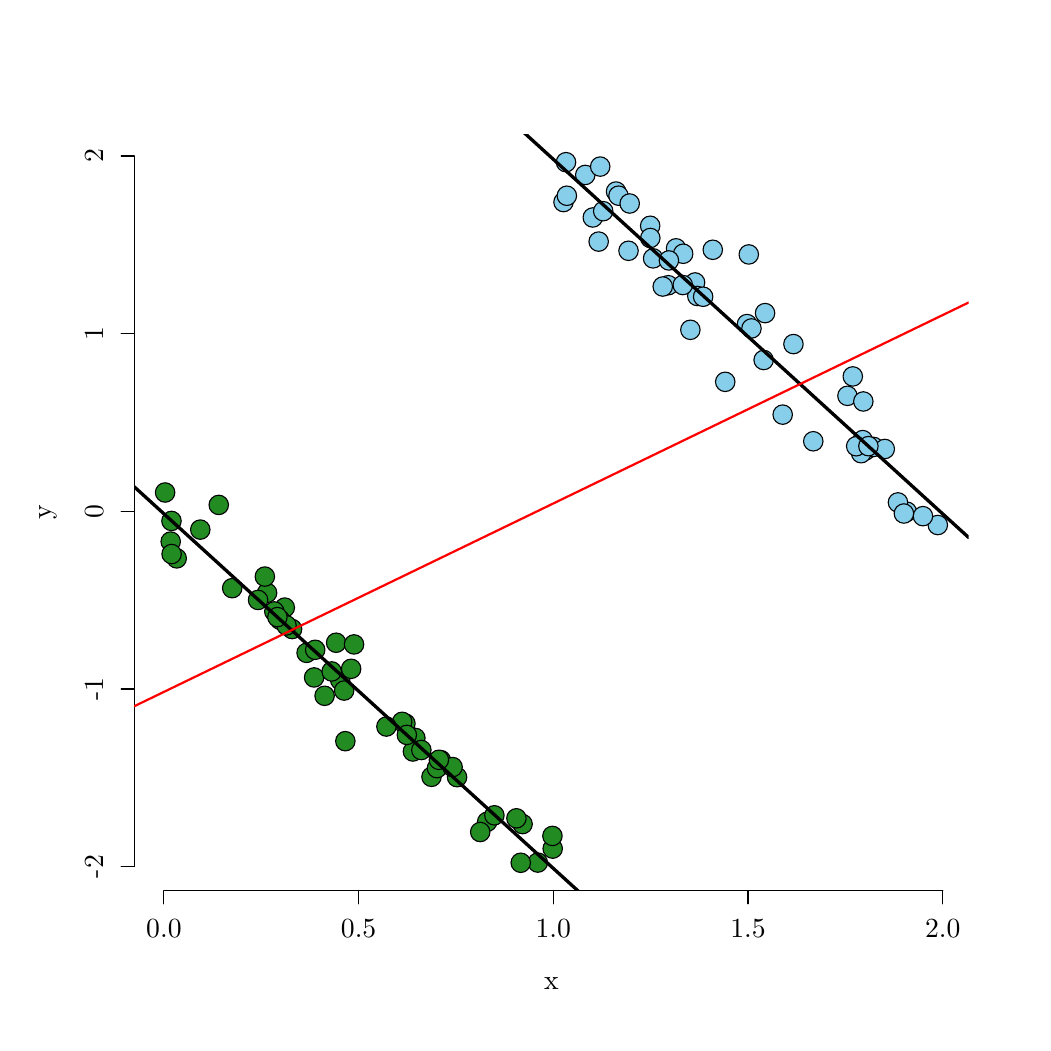
\begin{tikzpicture}[scale = 0.025]
% Created by tikzDevice version 0.10.1 on 2016-04-10 00:22:30
% !TEX encoding = UTF-8 Unicode
\definecolor{fillColor}{RGB}{255,255,255}
\path[use as bounding box,fill=fillColor,fill opacity=0.00] (0,0) rectangle (505.89,505.89);
\begin{scope}
\path[clip] (  0.00,  0.00) rectangle (505.89,505.89);
\definecolor{drawColor}{RGB}{0,0,0}

\path[draw=drawColor,line width= 0.4pt,line join=round,line cap=round] ( 69.23, 67.32) -- (464.96, 67.32);

\path[draw=drawColor,line width= 0.4pt,line join=round,line cap=round] ( 69.23, 67.32) -- ( 69.23, 60.72);

\path[draw=drawColor,line width= 0.4pt,line join=round,line cap=round] (168.16, 67.32) -- (168.16, 60.72);

\path[draw=drawColor,line width= 0.4pt,line join=round,line cap=round] (267.10, 67.32) -- (267.10, 60.72);

\path[draw=drawColor,line width= 0.4pt,line join=round,line cap=round] (366.03, 67.32) -- (366.03, 60.72);

\path[draw=drawColor,line width= 0.4pt,line join=round,line cap=round] (464.96, 67.32) -- (464.96, 60.72);

\node[text=drawColor,anchor=base,inner sep=0pt, outer sep=0pt, scale=  1.00] at ( 69.23, 43.56) {0.0};

\node[text=drawColor,anchor=base,inner sep=0pt, outer sep=0pt, scale=  1.00] at (168.16, 43.56) {0.5};

\node[text=drawColor,anchor=base,inner sep=0pt, outer sep=0pt, scale=  1.00] at (267.10, 43.56) {1.0};

\node[text=drawColor,anchor=base,inner sep=0pt, outer sep=0pt, scale=  1.00] at (366.03, 43.56) {1.5};

\node[text=drawColor,anchor=base,inner sep=0pt, outer sep=0pt, scale=  1.00] at (464.96, 43.56) {2.0};

\path[draw=drawColor,line width= 0.4pt,line join=round,line cap=round] ( 54.12, 79.57) -- ( 54.12,440.69);

\path[draw=drawColor,line width= 0.4pt,line join=round,line cap=round] ( 54.12, 79.57) -- ( 47.52, 79.57);

\path[draw=drawColor,line width= 0.4pt,line join=round,line cap=round] ( 54.12,169.85) -- ( 47.52,169.85);

\path[draw=drawColor,line width= 0.4pt,line join=round,line cap=round] ( 54.12,260.13) -- ( 47.52,260.13);

\path[draw=drawColor,line width= 0.4pt,line join=round,line cap=round] ( 54.12,350.41) -- ( 47.52,350.41);

\path[draw=drawColor,line width= 0.4pt,line join=round,line cap=round] ( 54.12,440.69) -- ( 47.52,440.69);

\node[text=drawColor,rotate= 90.00,anchor=base,inner sep=0pt, outer sep=0pt, scale=  1.00] at ( 38.28, 79.57) {-2};

\node[text=drawColor,rotate= 90.00,anchor=base,inner sep=0pt, outer sep=0pt, scale=  1.00] at ( 38.28,169.85) {-1};

\node[text=drawColor,rotate= 90.00,anchor=base,inner sep=0pt, outer sep=0pt, scale=  1.00] at ( 38.28,260.13) {0};

\node[text=drawColor,rotate= 90.00,anchor=base,inner sep=0pt, outer sep=0pt, scale=  1.00] at ( 38.28,350.41) {1};

\node[text=drawColor,rotate= 90.00,anchor=base,inner sep=0pt, outer sep=0pt, scale=  1.00] at ( 38.28,440.69) {2};
\end{scope}
\begin{scope}
\path[clip] (  0.00,  0.00) rectangle (505.89,505.89);
\definecolor{drawColor}{RGB}{0,0,0}

\node[text=drawColor,anchor=base,inner sep=0pt, outer sep=0pt, scale=  1.00] at (266.14, 17.16) {x};

\node[text=drawColor,rotate= 90.00,anchor=base,inner sep=0pt, outer sep=0pt, scale=  1.00] at ( 11.88,259.55) {y};
\end{scope}
\begin{scope}
\path[clip] ( 54.12, 67.32) rectangle (478.17,451.77);
\definecolor{drawColor}{RGB}{0,0,0}
\definecolor{fillColor}{RGB}{34,139,34}

\path[draw=drawColor,line width= 0.4pt,line join=round,line cap=round,fill=fillColor] (191.95,152.28) circle (  4.95);

\path[draw=drawColor,line width= 0.4pt,line join=round,line cap=round,fill=fillColor] (233.48,102.37) circle (  4.95);

\path[draw=drawColor,line width= 0.4pt,line join=round,line cap=round,fill=fillColor] (196.99,144.98) circle (  4.95);

\path[draw=drawColor,line width= 0.4pt,line join=round,line cap=round,fill=fillColor] ( 75.73,236.22) circle (  4.95);

\path[draw=drawColor,line width= 0.4pt,line join=round,line cap=round,fill=fillColor] (121.65,218.70) circle (  4.95);

\path[draw=drawColor,line width= 0.4pt,line join=round,line cap=round,fill=fillColor] (209.94,133.71) circle (  4.95);

\path[draw=drawColor,line width= 0.4pt,line join=round,line cap=round,fill=fillColor] ( 97.09,263.39) circle (  4.95);

\path[draw=drawColor,line width= 0.4pt,line join=round,line cap=round,fill=fillColor] (190.29,153.19) circle (  4.95);

\path[draw=drawColor,line width= 0.4pt,line join=round,line cap=round,fill=fillColor] (150.87,166.40) circle (  4.95);

\path[draw=drawColor,line width= 0.4pt,line join=round,line cap=round,fill=fillColor] ( 72.67,244.76) circle (  4.95);

\path[draw=drawColor,line width= 0.4pt,line join=round,line cap=round,fill=fillColor] (158.80,174.40) circle (  4.95);

\path[draw=drawColor,line width= 0.4pt,line join=round,line cap=round,fill=fillColor] (229.95, 97.18) circle (  4.95);

\path[draw=drawColor,line width= 0.4pt,line join=round,line cap=round,fill=fillColor] (145.55,175.73) circle (  4.95);

\path[draw=drawColor,line width= 0.4pt,line join=round,line cap=round,fill=fillColor] (259.20, 81.65) circle (  4.95);

\path[draw=drawColor,line width= 0.4pt,line join=round,line cap=round,fill=fillColor] (103.93,221.09) circle (  4.95);

\path[draw=drawColor,line width= 0.4pt,line join=round,line cap=round,fill=fillColor] ( 87.71,250.84) circle (  4.95);

\path[draw=drawColor,line width= 0.4pt,line join=round,line cap=round,fill=fillColor] (205.20,125.22) circle (  4.95);

\path[draw=drawColor,line width= 0.4pt,line join=round,line cap=round,fill=fillColor] (141.72,188.22) circle (  4.95);

\path[draw=drawColor,line width= 0.4pt,line join=round,line cap=round,fill=fillColor] (250.54, 81.56) circle (  4.95);

\path[draw=drawColor,line width= 0.4pt,line join=round,line cap=round,fill=fillColor] (164.36,180.11) circle (  4.95);

\path[draw=drawColor,line width= 0.4pt,line join=round,line cap=round,fill=fillColor] (117.06,215.10) circle (  4.95);

\path[draw=drawColor,line width= 0.4pt,line join=round,line cap=round,fill=fillColor] (251.47,101.21) circle (  4.95);

\path[draw=drawColor,line width= 0.4pt,line join=round,line cap=round,fill=fillColor] (195.75,138.10) circle (  4.95);

\path[draw=drawColor,line width= 0.4pt,line join=round,line cap=round,fill=fillColor] (200.04,138.85) circle (  4.95);

\path[draw=drawColor,line width= 0.4pt,line join=round,line cap=round,fill=fillColor] (130.65,211.23) circle (  4.95);

\path[draw=drawColor,line width= 0.4pt,line join=round,line cap=round,fill=fillColor] (128.21,205.04) circle (  4.95);

\path[draw=drawColor,line width= 0.4pt,line join=round,line cap=round,fill=fillColor] (266.77, 88.75) circle (  4.95);

\path[draw=drawColor,line width= 0.4pt,line join=round,line cap=round,fill=fillColor] (218.18,125.04) circle (  4.95);

\path[draw=drawColor,line width= 0.4pt,line join=round,line cap=round,fill=fillColor] (182.28,150.78) circle (  4.95);

\path[draw=drawColor,line width= 0.4pt,line join=round,line cap=round,fill=fillColor] ( 73.07,255.25) circle (  4.95);

\path[draw=drawColor,line width= 0.4pt,line join=round,line cap=round,fill=fillColor] (160.82,169.06) circle (  4.95);

\path[draw=drawColor,line width= 0.4pt,line join=round,line cap=round,fill=fillColor] (156.74,193.36) circle (  4.95);

\path[draw=drawColor,line width= 0.4pt,line join=round,line cap=round,fill=fillColor] (192.66,146.52) circle (  4.95);

\path[draw=drawColor,line width= 0.4pt,line join=round,line cap=round,fill=fillColor] (120.51,226.98) circle (  4.95);

\path[draw=drawColor,line width= 0.4pt,line join=round,line cap=round,fill=fillColor] (207.96,129.64) circle (  4.95);

\path[draw=drawColor,line width= 0.4pt,line join=round,line cap=round,fill=fillColor] ( 69.83,269.70) circle (  4.95);

\path[draw=drawColor,line width= 0.4pt,line join=round,line cap=round,fill=fillColor] (146.10,189.77) circle (  4.95);

\path[draw=drawColor,line width= 0.4pt,line join=round,line cap=round,fill=fillColor] (215.92,130.19) circle (  4.95);

\path[draw=drawColor,line width= 0.4pt,line join=round,line cap=round,fill=fillColor] (266.64, 95.20) circle (  4.95);

\path[draw=drawColor,line width= 0.4pt,line join=round,line cap=round,fill=fillColor] (161.42,143.34) circle (  4.95);

\path[draw=drawColor,line width= 0.4pt,line join=round,line cap=round,fill=fillColor] (165.84,192.50) circle (  4.95);

\path[draw=drawColor,line width= 0.4pt,line join=round,line cap=round,fill=fillColor] (125.31,209.27) circle (  4.95);

\path[draw=drawColor,line width= 0.4pt,line join=round,line cap=round,fill=fillColor] (134.36,200.31) circle (  4.95);

\path[draw=drawColor,line width= 0.4pt,line join=round,line cap=round,fill=fillColor] (131.50,202.18) circle (  4.95);

\path[draw=drawColor,line width= 0.4pt,line join=round,line cap=round,fill=fillColor] (237.15,105.67) circle (  4.95);

\path[draw=drawColor,line width= 0.4pt,line join=round,line cap=round,fill=fillColor] (208.95,133.87) circle (  4.95);

\path[draw=drawColor,line width= 0.4pt,line join=round,line cap=round,fill=fillColor] (126.89,206.40) circle (  4.95);

\path[draw=drawColor,line width= 0.4pt,line join=round,line cap=round,fill=fillColor] (154.46,178.78) circle (  4.95);

\path[draw=drawColor,line width= 0.4pt,line join=round,line cap=round,fill=fillColor] (248.35,104.15) circle (  4.95);

\path[draw=drawColor,line width= 0.4pt,line join=round,line cap=round,fill=fillColor] ( 73.13,238.43) circle (  4.95);
\definecolor{fillColor}{RGB}{135,206,235}

\path[draw=drawColor,line width= 0.4pt,line join=round,line cap=round,fill=fillColor] (339.11,376.42) circle (  4.95);

\path[draw=drawColor,line width= 0.4pt,line join=round,line cap=round,fill=fillColor] (305.30,392.52) circle (  4.95);

\path[draw=drawColor,line width= 0.4pt,line join=round,line cap=round,fill=fillColor] (340.25,369.55) circle (  4.95);

\path[draw=drawColor,line width= 0.4pt,line join=round,line cap=round,fill=fillColor] (316.31,405.22) circle (  4.95);

\path[draw=drawColor,line width= 0.4pt,line join=round,line cap=round,fill=fillColor] (365.50,355.28) circle (  4.95);

\path[draw=drawColor,line width= 0.4pt,line join=round,line cap=round,fill=fillColor] (298.96,422.62) circle (  4.95);

\path[draw=drawColor,line width= 0.4pt,line join=round,line cap=round,fill=fillColor] (272.27,417.27) circle (  4.95);

\path[draw=drawColor,line width= 0.4pt,line join=round,line cap=round,fill=fillColor] (446.73,259.94) circle (  4.95);

\path[draw=drawColor,line width= 0.4pt,line join=round,line cap=round,fill=fillColor] (290.13,397.19) circle (  4.95);

\path[draw=drawColor,line width= 0.4pt,line join=round,line cap=round,fill=fillColor] (416.54,318.82) circle (  4.95);

\path[draw=drawColor,line width= 0.4pt,line join=round,line cap=round,fill=fillColor] (336.73,352.36) circle (  4.95);

\path[draw=drawColor,line width= 0.4pt,line join=round,line cap=round,fill=fillColor] (442.21,264.66) circle (  4.95);

\path[draw=drawColor,line width= 0.4pt,line join=round,line cap=round,fill=fillColor] (287.15,409.44) circle (  4.95);

\path[draw=drawColor,line width= 0.4pt,line join=round,line cap=round,fill=fillColor] (300.22,420.52) circle (  4.95);

\path[draw=drawColor,line width= 0.4pt,line join=round,line cap=round,fill=fillColor] (317.80,388.67) circle (  4.95);

\path[draw=drawColor,line width= 0.4pt,line join=round,line cap=round,fill=fillColor] (425.87,291.18) circle (  4.95);

\path[draw=drawColor,line width= 0.4pt,line join=round,line cap=round,fill=fillColor] (348.11,393.03) circle (  4.95);

\path[draw=drawColor,line width= 0.4pt,line join=round,line cap=round,fill=fillColor] (329.45,393.77) circle (  4.95);

\path[draw=drawColor,line width= 0.4pt,line join=round,line cap=round,fill=fillColor] (424.30,296.32) circle (  4.95);

\path[draw=drawColor,line width= 0.4pt,line join=round,line cap=round,fill=fillColor] (366.41,390.66) circle (  4.95);

\path[draw=drawColor,line width= 0.4pt,line join=round,line cap=round,fill=fillColor] (424.61,315.95) circle (  4.95);

\path[draw=drawColor,line width= 0.4pt,line join=round,line cap=round,fill=fillColor] (354.44,325.93) circle (  4.95);

\path[draw=drawColor,line width= 0.4pt,line join=round,line cap=round,fill=fillColor] (333.08,391.01) circle (  4.95);

\path[draw=drawColor,line width= 0.4pt,line join=round,line cap=round,fill=fillColor] (389.10,345.11) circle (  4.95);

\path[draw=drawColor,line width= 0.4pt,line join=round,line cap=round,fill=fillColor] (383.64,309.27) circle (  4.95);

\path[draw=drawColor,line width= 0.4pt,line join=round,line cap=round,fill=fillColor] (273.54,437.53) circle (  4.95);

\path[draw=drawColor,line width= 0.4pt,line join=round,line cap=round,fill=fillColor] (462.46,253.17) circle (  4.95);

\path[draw=drawColor,line width= 0.4pt,line join=round,line cap=round,fill=fillColor] (305.90,416.54) circle (  4.95);

\path[draw=drawColor,line width= 0.4pt,line join=round,line cap=round,fill=fillColor] (373.96,337.02) circle (  4.95);

\path[draw=drawColor,line width= 0.4pt,line join=round,line cap=round,fill=fillColor] (325.82,387.61) circle (  4.95);

\path[draw=drawColor,line width= 0.4pt,line join=round,line cap=round,fill=fillColor] (283.32,431.05) circle (  4.95);

\path[draw=drawColor,line width= 0.4pt,line join=round,line cap=round,fill=fillColor] (429.87,292.84) circle (  4.95);

\path[draw=drawColor,line width= 0.4pt,line join=round,line cap=round,fill=fillColor] (325.52,375.02) circle (  4.95);

\path[draw=drawColor,line width= 0.4pt,line join=round,line cap=round,fill=fillColor] (399.17,295.73) circle (  4.95);

\path[draw=drawColor,line width= 0.4pt,line join=round,line cap=round,fill=fillColor] (454.91,257.68) circle (  4.95);

\path[draw=drawColor,line width= 0.4pt,line join=round,line cap=round,fill=fillColor] (374.68,360.85) circle (  4.95);

\path[draw=drawColor,line width= 0.4pt,line join=round,line cap=round,fill=fillColor] (332.88,375.12) circle (  4.95);

\path[draw=drawColor,line width= 0.4pt,line join=round,line cap=round,fill=fillColor] (419.26,328.68) circle (  4.95);

\path[draw=drawColor,line width= 0.4pt,line join=round,line cap=round,fill=fillColor] (290.92,435.30) circle (  4.95);

\path[draw=drawColor,line width= 0.4pt,line join=round,line cap=round,fill=fillColor] (273.97,420.49) circle (  4.95);

\path[draw=drawColor,line width= 0.4pt,line join=round,line cap=round,fill=fillColor] (423.49,289.66) circle (  4.95);

\path[draw=drawColor,line width= 0.4pt,line join=round,line cap=round,fill=fillColor] (322.69,374.36) circle (  4.95);

\path[draw=drawColor,line width= 0.4pt,line join=round,line cap=round,fill=fillColor] (367.78,353.05) circle (  4.95);

\path[draw=drawColor,line width= 0.4pt,line join=round,line cap=round,fill=fillColor] (292.44,412.64) circle (  4.95);

\path[draw=drawColor,line width= 0.4pt,line join=round,line cap=round,fill=fillColor] (343.22,369.17) circle (  4.95);

\path[draw=drawColor,line width= 0.4pt,line join=round,line cap=round,fill=fillColor] (445.22,259.02) circle (  4.95);

\path[draw=drawColor,line width= 0.4pt,line join=round,line cap=round,fill=fillColor] (420.99,293.20) circle (  4.95);

\path[draw=drawColor,line width= 0.4pt,line join=round,line cap=round,fill=fillColor] (435.51,291.81) circle (  4.95);

\path[draw=drawColor,line width= 0.4pt,line join=round,line cap=round,fill=fillColor] (316.38,399.01) circle (  4.95);

\path[draw=drawColor,line width= 0.4pt,line join=round,line cap=round,fill=fillColor] (427.19,293.25) circle (  4.95);

\path[draw=drawColor,line width= 1.2pt,line join=round,line cap=round] ( 54.12,272.63) -- (353.51,  0.00);

\path[draw=drawColor,line width= 1.2pt,line join=round,line cap=round] (193.64,505.89) -- (478.17,246.79);
\definecolor{drawColor}{RGB}{255,0,0}

\path[draw=drawColor,line width= 0.8pt,line join=round,line cap=round] ( 54.12,161.07) -- (478.17,366.26);
\end{scope}

\end{tikzpicture}
\end{center}
\end{minipage}

\item А вот так не бывает!
\end{enumerate}
\end{sol}
\end{problem}




\begin{problem} %1.16
Вася оценил модель $y=\beta_1+\beta_2 d+\beta_3 x+\varepsilon$. Дамми-переменная $d$ обозначает пол, 1 для мужчин и 0 для женщин. Оказалось, что $\hb_2>0$. Означает ли это, что для мужчин $\bar{y}$ больше, чем $\bar{y}$ для женщин?


\begin{sol}
Нет. Коэффициенты можно интерпретировать только «при прочих равных», т.е. при равных $x$. Из-за разных $x$ может оказаться, что у мужчин $\bar{y}$ меньше, чем $\bar{y}$ для женщин.
\end{sol}
\end{problem}




\begin{problem} %1.17
Какие из указанные моделей можно представить в линейном виде?
\begin{enumerate}
\item $y_i=\beta_1+\frac{\beta_2}{x_i}+\e_i$;
\item $y_i=\exp(\beta_1+\beta_2 x_i+\e_i)$;
\item $y_i=1+\frac{1}{\exp(\beta_1+\beta_2 x_i+\e_i)}$;
\item $y_i=\frac{1}{1+\exp(\beta_1+\beta_2 x_i+\e_i)}$;
\item $y_i=x_i^{\beta_2}e^{\beta_1+\e_i}$;
\item $y_i=\beta_1\exp(\beta_2 x_i + \e_i)$.
\end{enumerate}


\begin{sol}
Модель можно представить в линейном виде, когда неизвестные параметры входят в нее линейно.
\begin{enumerate}
\item Обозначим $z_i = 1/x_i$, и готово.
\item Возьмем логарифм от обеих частей\ldots
\item Вычтем единицу из обеих частей и снова логарифм\ldots
\item Перевернем обе части уравнения, вычтем единицу и прологарифмируем\ldots
\item Вместо $x_i$ возьмем $e^{x_i}$ и прологарифмируем\ldots
\item Вместо $\beta_1$ возьмем $e^{\beta_1}$ и прологарифмируем\ldots
\end{enumerate}
\end{sol}
\end{problem}




\begin{problem} %1.18
У эконометриста Вовочки есть переменная $f_i$, которая равна 1, если $i$-ый человек в выборке — женщина, и 0, если мужчина. Есть переменная $m_i$, которая равна 1, если $i$-ый человек в выборке — мужчина, и 0, если женщина. Какие $\hy$ получатся, если Вовочка попытается построить регрессии:
\begin{enumerate}
\item $y$ на константу и $f$;
\item $y$ на константу и $m$;
\item $y$ на $f$ и $m$ без константы;
\item $y$ на константу, $f$ и $m$.
\end{enumerate}


\begin{sol}
Пусть \(\bar{y}_m\) — среднее значение \(y\) по выборке для мужчин, \(\bar{y}_f\) — среднее значение \(y\) по выборке для женщин. Тогда

\begin{enumerate}
\item \(\hy = \bar{y}_m + \left( \bar{y}_m -  \bar{y}_f \right) \cdot f \)

Оцениваемая модель:
\[
y_i = \beta_1 + \beta_2 f_i + \e_i 
\]

Стандартная процедура МНК:
\[RSS = \sum \e_i^2 = \sum \left(y_i - \beta_1 - \beta_2 \cdot f_i \right)^2 \rightarrow \min \limits_{\beta_1, \beta_2}\]
\[\frac{\partial RSS}{\partial \beta_1} = 2 \sum \left(y_i - \beta_1 - \beta_2\right)(-1) \]
\[\frac{\partial RSS}{\partial \beta_2} = 2 \sum \left(y_i - \beta_1 - \beta_2 \right)(-f_i) \]

Условия первого порядка:
\[\sum \left(y_i - \hb_1 - \hb_2 \cdot f_i\right) = 0\]
\[\sum \left(\left(y_i - \hb_1 - \hb_2 \cdot f_i\right)\cdot f_i\right)= 0\]

Осталось немного поработать с оператором суммирования. Обозначим за \(k\) — число женщин в нашей выборке объемом \(n\), мужчин тогда будет \(n - k\). Тогда
\[\sum \left(y_i - \hb_1 - \hb_2 \cdot f_i\right) = k \bar{y}_f + (n - k) \bar{y}_m - n \hb_1 - k \hb_2 = 0\]
\[\sum \left(\left(y_i - \hb_1 - \hb_2 \cdot f_i\right)\cdot f_i\right) = k \bar{y}_f - k \hb_1 - k \hb_2 =0\]

Отсюда легко ищутся оценки коэффициентов:
\[\hb_1 = \bar{y}_m, \ \hb_2 = \bar{y}_f - \bar{y}_m  \]

Следовательно:
\[\hy = \bar{y}_m + \left( \bar{y}_f -  \bar{y}_m \right) \cdot f \]

\item \(\hy = \bar{y}_f + \left( \bar{y}_m -  \bar{y}_f \right) \cdot m \)

\item \(\hy = \bar{y}_m \cdot m + \bar{y}_f \cdot f \)

\item Условия первого порядка линейного зависимы — мультиколлинеарность. МНК-оценки здесь не единственны.
\end{enumerate}
\end{sol}
\end{problem}




\begin{problem} %1.19
У эконометриста Вовочки есть три переменных: $r_i$ — доход $i$-го человека в выборке, $m_i$ — пол (1 — мальчик, 0 — девочка) и $f_i$ — пол (1 — девочка, 0 — мальчик). Вовочка оценил две модели
\begin{enumerate}
\item[] Модель A: $m_i=\beta_1+\beta_2 r_i+\ve_i$;
\item[] Модель B: $f_i=\gamma_1+\gamma_2 r_i+u_i$.
\end{enumerate}
\begin{enumerate}
\item Как связаны между собой оценки $\hb_1$ и $\hat{\gamma}_1$?
\item Как связаны между собой оценки $\hb_2$ и $\hat{\gamma}_2$?
\end{enumerate}


\begin{sol}
Если сложить попарно $m_i$ и $f_i$, то в сумме всегда выйдет единица. А оценки, полученные при помощи метода наименьших квадратов линейны по объясняемой переменной, то есть оценки коэффициентов модели $m_i+f_i \sim \dots$ это суммы соответствующих оценок из двух разных моделей. Но они должны получиться равными 1 и 0 соответствнно (так как зависимая переменная — вектор из единиц). Поэтому $\hb_1 + \hat{\gamma}_1 = 1$, $\hb_2 + \hat{\gamma}_2 = 0$.
\end{sol}
\end{problem}




\begin{problem} %1.20
Эконометрист Вовочка оценил линейную регрессионную модель, где $y$ измерялся в тугриках. Затем он оценил ту же модель, но измерял $y$ в мунгу (1 тугрик = 100 мунгу). Как изменятся оценки коэффициентов?


\begin{sol}
Все оценки коэффициентов увеличатся в 100 раз.
\end{sol}
\end{problem}



\begin{problem} %1.21
Возможно ли, что при оценке парной регрессии $y=\beta_1+\beta_2 x+\e$ оказывается, что $\hb_2>0$, а при оценке регрессии без константы, $y=\gamma x+\e$, оказывается, что $\hat{\gamma}<0$?


\begin{sol}
Да, возможно:

\begin{minted}[mathescape,
               linenos,
               numbersep=5pt,
               frame=lines,
               framesep=2mm]{r}
tikz("../R_plots/with_and_without_c.tikz", standAlone = FALSE, bareBones = TRUE)
x <- c(rnorm(n, mean = 4, sd = 2))
y <- x - 7 + runif(n, min = -1, max = 1)

plot(x,y, pch = 21, bg = "ForestGreen",
     col = "black", xlim = c(0,10), ylim = c(-5,3))
abline(coef(lm(y ~ x))[1], coef(lm(y ~ x))[2], lwd = 2)
abline(0, coef(lm(y ~ 0 + x))[1] , lwd = 2)
labels <- c("With intercept", "Without intercept")
text(c(7.5, 1.5), c(2, 0.4), labels)
coef(lm(y ~ x))
coef(lm(y ~ 0 + x))
invisible(dev.off())
\end{minted}

\begin{minipage}{0.6\textwidth}
\begin{center}
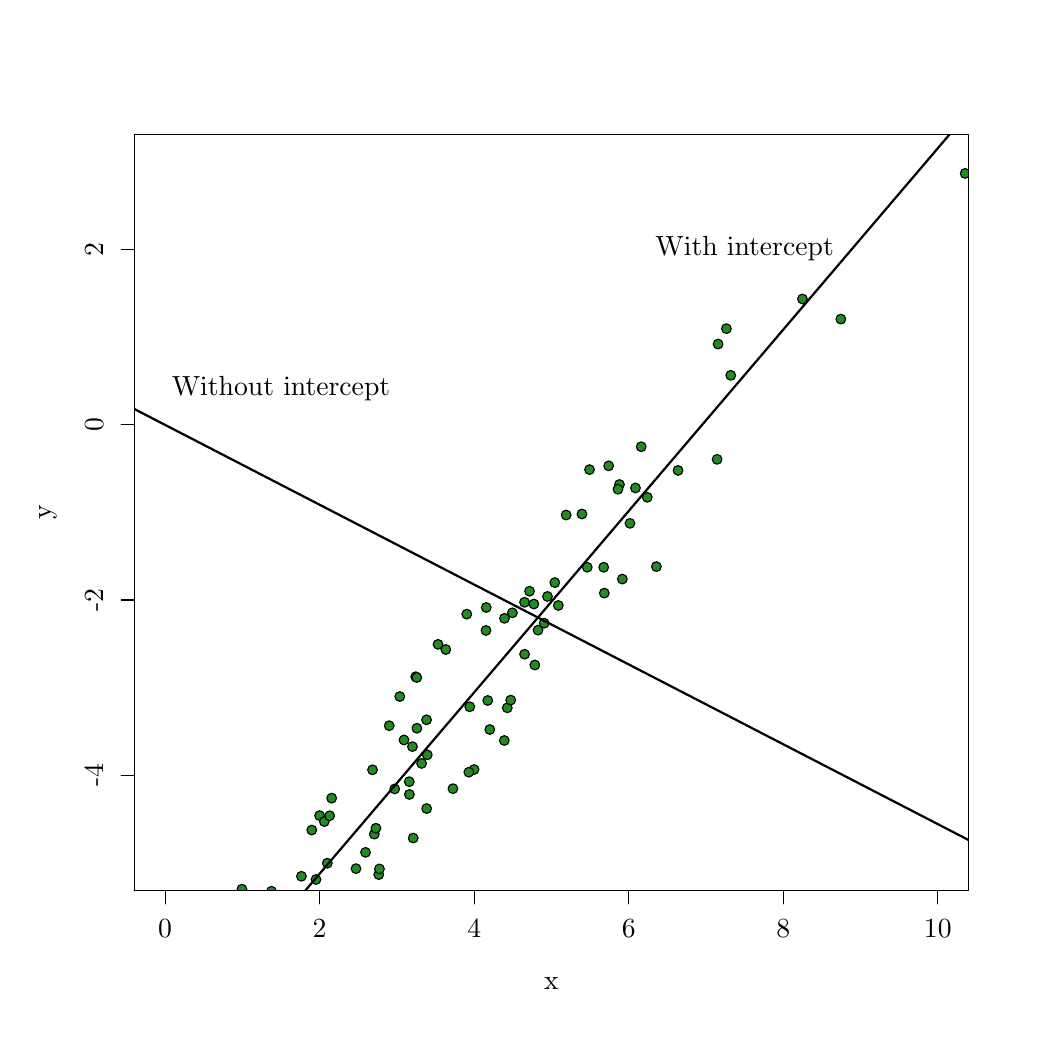
\begin{tikzpicture}[scale = 0.025]
% Created by tikzDevice version 0.10.1 on 2016-04-10 00:22:30
% !TEX encoding = UTF-8 Unicode
\definecolor{fillColor}{RGB}{255,255,255}
\path[use as bounding box,fill=fillColor,fill opacity=0.00] (0,0) rectangle (505.89,505.89);
\begin{scope}
\path[clip] ( 54.12, 67.32) rectangle (478.17,451.77);
\definecolor{drawColor}{RGB}{0,0,0}
\definecolor{fillColor}{RGB}{34,139,34}

\path[draw=drawColor,line width= 0.4pt,line join=round,line cap=round,fill=fillColor] (162.52, 64.24) circle (  2.47);

\path[draw=drawColor,line width= 0.4pt,line join=round,line cap=round,fill=fillColor] (314.84,267.24) circle (  2.47);

\path[draw=drawColor,line width= 0.4pt,line join=round,line cap=round,fill=fillColor] (216.09,119.22) circle (  2.47);

\path[draw=drawColor,line width= 0.4pt,line join=round,line cap=round,fill=fillColor] (175.23,128.78) circle (  2.47);

\path[draw=drawColor,line width= 0.4pt,line join=round,line cap=round,fill=fillColor] (257.69,182.04) circle (  2.47);

\path[draw=drawColor,line width= 0.4pt,line join=round,line cap=round,fill=fillColor] (197.19,176.09) circle (  2.47);

\path[draw=drawColor,line width= 0.4pt,line join=round,line cap=round,fill=fillColor] (226.83,128.94) circle (  2.47);

\path[draw=drawColor,line width= 0.4pt,line join=round,line cap=round,fill=fillColor] (295.21,283.25) circle (  2.47);

\path[draw=drawColor,line width= 0.4pt,line join=round,line cap=round,fill=fillColor] (357.25,329.23) circle (  2.47);

\path[draw=drawColor,line width= 0.4pt,line join=round,line cap=round,fill=fillColor] (200.17,132.03) circle (  2.47);

\path[draw=drawColor,line width= 0.4pt,line join=round,line cap=round,fill=fillColor] (476.34,431.84) circle (  2.47);

\path[draw=drawColor,line width= 0.4pt,line join=round,line cap=round,fill=fillColor] (183.72,151.21) circle (  2.47);

\path[draw=drawColor,line width= 0.4pt,line join=round,line cap=round,fill=fillColor] (269.64,212.31) circle (  2.47);

\path[draw=drawColor,line width= 0.4pt,line join=round,line cap=round,fill=fillColor] (284.33,231.72) circle (  2.47);

\path[draw=drawColor,line width= 0.4pt,line join=round,line cap=round,fill=fillColor] (350.82,345.12) circle (  2.47);

\path[draw=drawColor,line width= 0.4pt,line join=round,line cap=round,fill=fillColor] (176.14, 96.11) circle (  2.47);

\path[draw=drawColor,line width= 0.4pt,line join=round,line cap=round,fill=fillColor] (178.39, 75.55) circle (  2.47);

\path[draw=drawColor,line width= 0.4pt,line join=round,line cap=round,fill=fillColor] (257.19,213.04) circle (  2.47);

\path[draw=drawColor,line width= 0.4pt,line join=round,line cap=round,fill=fillColor] (302.16,225.71) circle (  2.47);

\path[draw=drawColor,line width= 0.4pt,line join=round,line cap=round,fill=fillColor] (319.47,232.04) circle (  2.47);

\path[draw=drawColor,line width= 0.4pt,line join=round,line cap=round,fill=fillColor] (195.52,140.57) circle (  2.47);

\path[draw=drawColor,line width= 0.4pt,line join=round,line cap=round,fill=fillColor] (262.45,203.28) circle (  2.47);

\path[draw=drawColor,line width= 0.4pt,line join=round,line cap=round,fill=fillColor] (292.68,231.70) circle (  2.47);

\path[draw=drawColor,line width= 0.4pt,line join=round,line cap=round,fill=fillColor] (242.18,143.68) circle (  2.47);

\path[draw=drawColor,line width= 0.4pt,line join=round,line cap=round,fill=fillColor] (252.46,213.90) circle (  2.47);

\path[draw=drawColor,line width= 0.4pt,line join=round,line cap=round,fill=fillColor] (197.73,175.69) circle (  2.47);

\path[draw=drawColor,line width= 0.4pt,line join=round,line cap=round,fill=fillColor] (154.46,114.39) circle (  2.47);

\path[draw=drawColor,line width= 0.4pt,line join=round,line cap=round,fill=fillColor] (202.69,154.19) circle (  2.47);

\path[draw=drawColor,line width= 0.4pt,line join=round,line cap=round,fill=fillColor] (108.87, 68.13) circle (  2.47);

\path[draw=drawColor,line width= 0.4pt,line join=round,line cap=round,fill=fillColor] (193.95,116.27) circle (  2.47);

\path[draw=drawColor,line width= 0.4pt,line join=round,line cap=round,fill=fillColor] (232.89,199.60) circle (  2.47);

\path[draw=drawColor,line width= 0.4pt,line join=round,line cap=round,fill=fillColor] (137.46, 28.79) circle (  2.47);

\path[draw=drawColor,line width= 0.4pt,line join=round,line cap=round,fill=fillColor] (293.00,218.57) circle (  2.47);

\path[draw=drawColor,line width= 0.4pt,line join=round,line cap=round,fill=fillColor] (264.11,216.87) circle (  2.47);

\path[draw=drawColor,line width= 0.4pt,line join=round,line cap=round,fill=fillColor] (151.04, 54.46) circle (  2.47);

\path[draw=drawColor,line width= 0.4pt,line join=round,line cap=round,fill=fillColor] (259.34,199.75) circle (  2.47);

\path[draw=drawColor,line width= 0.4pt,line join=round,line cap=round,fill=fillColor] (246.30,208.55) circle (  2.47);

\path[draw=drawColor,line width= 0.4pt,line join=round,line cap=round,fill=fillColor] (281.64,258.77) circle (  2.47);

\path[draw=drawColor,line width= 0.4pt,line join=round,line cap=round,fill=fillColor] (186.50,119.08) circle (  2.47);

\path[draw=drawColor,line width= 0.4pt,line join=round,line cap=round,fill=fillColor] (131.05, 22.55) circle (  2.47);

\path[draw=drawColor,line width= 0.4pt,line join=round,line cap=round,fill=fillColor] (134.37, 58.47) circle (  2.47);

\path[draw=drawColor,line width= 0.4pt,line join=round,line cap=round,fill=fillColor] (212.46,189.92) circle (  2.47);

\path[draw=drawColor,line width= 0.4pt,line join=round,line cap=round,fill=fillColor] (203.04,136.40) circle (  2.47);

\path[draw=drawColor,line width= 0.4pt,line join=round,line cap=round,fill=fillColor] (123.88, 67.09) circle (  2.47);

\path[draw=drawColor,line width= 0.4pt,line join=round,line cap=round,fill=fillColor] ( 89.55, 23.87) circle (  2.47);

\path[draw=drawColor,line width= 0.4pt,line join=round,line cap=round,fill=fillColor] (224.63,160.82) circle (  2.47);

\path[draw=drawColor,line width= 0.4pt,line join=round,line cap=round,fill=fillColor] (109.78, 12.27) circle (  2.47);

\path[draw=drawColor,line width= 0.4pt,line join=round,line cap=round,fill=fillColor] (273.62,258.26) circle (  2.47);

\path[draw=drawColor,line width= 0.4pt,line join=round,line cap=round,fill=fillColor] (178.74, 78.43) circle (  2.47);

\path[draw=drawColor,line width= 0.4pt,line join=round,line cap=round,fill=fillColor] (252.49,187.52) circle (  2.47);

\path[draw=drawColor,line width= 0.4pt,line join=round,line cap=round,fill=fillColor] (197.76,149.91) circle (  2.47);

\path[draw=drawColor,line width= 0.4pt,line join=round,line cap=round,fill=fillColor] (125.93, 63.57) circle (  2.47);

\path[draw=drawColor,line width= 0.4pt,line join=round,line cap=round,fill=fillColor] (132.63, 60.95) circle (  2.47);

\path[draw=drawColor,line width= 0.4pt,line join=round,line cap=round,fill=fillColor] (148.31,105.52) circle (  2.47);

\path[draw=drawColor,line width= 0.4pt,line join=round,line cap=round,fill=fillColor] (306.03,254.02) circle (  2.47);

\path[draw=drawColor,line width= 0.4pt,line join=round,line cap=round,fill=fillColor] (189.07,166.02) circle (  2.47);

\path[draw=drawColor,line width= 0.4pt,line join=round,line cap=round,fill=fillColor] (163.38, 60.24) circle (  2.47);

\path[draw=drawColor,line width= 0.4pt,line join=round,line cap=round,fill=fillColor] (224.16,127.58) circle (  2.47);

\path[draw=drawColor,line width= 0.4pt,line join=round,line cap=round,fill=fillColor] (150.74,102.49) circle (  2.47);

\path[draw=drawColor,line width= 0.4pt,line join=round,line cap=round,fill=fillColor] (145.01, 42.02) circle (  2.47);

\path[draw=drawColor,line width= 0.4pt,line join=round,line cap=round,fill=fillColor] (300.69,273.75) circle (  2.47);

\path[draw=drawColor,line width= 0.4pt,line join=round,line cap=round,fill=fillColor] (195.88, 94.12) circle (  2.47);

\path[draw=drawColor,line width= 0.4pt,line join=round,line cap=round,fill=fillColor] (145.55, 59.81) circle (  2.47);

\path[draw=drawColor,line width= 0.4pt,line join=round,line cap=round,fill=fillColor] (267.85,223.91) circle (  2.47);

\path[draw=drawColor,line width= 0.4pt,line join=round,line cap=round,fill=fillColor] (243.72,160.28) circle (  2.47);

\path[draw=drawColor,line width= 0.4pt,line join=round,line cap=round,fill=fillColor] (233.76,164.01) circle (  2.47);

\path[draw=drawColor,line width= 0.4pt,line join=round,line cap=round,fill=fillColor] (242.27,205.74) circle (  2.47);

\path[draw=drawColor,line width= 0.4pt,line join=round,line cap=round,fill=fillColor] (255.01,219.52) circle (  2.47);

\path[draw=drawColor,line width= 0.4pt,line join=round,line cap=round,fill=fillColor] (355.05,352.95) circle (  2.47);

\path[draw=drawColor,line width= 0.4pt,line join=round,line cap=round,fill=fillColor] (153.42,105.44) circle (  2.47);

\path[draw=drawColor,line width= 0.4pt,line join=round,line cap=round,fill=fillColor] (152.25, 81.31) circle (  2.47);

\path[draw=drawColor,line width= 0.4pt,line join=round,line cap=round,fill=fillColor] (144.35, 98.18) circle (  2.47);

\path[draw=drawColor,line width= 0.4pt,line join=round,line cap=round,fill=fillColor] (139.09, 74.69) circle (  2.47);

\path[draw=drawColor,line width= 0.4pt,line join=round,line cap=round,fill=fillColor] (191.22,143.95) circle (  2.47);

\path[draw=drawColor,line width= 0.4pt,line join=round,line cap=round,fill=fillColor] (234.81,149.26) circle (  2.47);

\path[draw=drawColor,line width= 0.4pt,line join=round,line cap=round,fill=fillColor] (413.18,357.81) circle (  2.47);

\path[draw=drawColor,line width= 0.4pt,line join=round,line cap=round,fill=fillColor] (146.51, 73.06) circle (  2.47);

\path[draw=drawColor,line width= 0.4pt,line join=round,line cap=round,fill=fillColor] (233.01,211.27) circle (  2.47);

\path[draw=drawColor,line width= 0.4pt,line join=round,line cap=round,fill=fillColor] (223.12,207.89) circle (  2.47);

\path[draw=drawColor,line width= 0.4pt,line join=round,line cap=round,fill=fillColor] (171.67, 86.83) circle (  2.47);

\path[draw=drawColor,line width= 0.4pt,line join=round,line cap=round,fill=fillColor] (330.47,280.91) circle (  2.47);

\path[draw=drawColor,line width= 0.4pt,line join=round,line cap=round,fill=fillColor] (139.92, 30.11) circle (  2.47);

\path[draw=drawColor,line width= 0.4pt,line join=round,line cap=round,fill=fillColor] (141.11, 48.30) circle (  2.47);

\path[draw=drawColor,line width= 0.4pt,line join=round,line cap=round,fill=fillColor] (245.45,164.21) circle (  2.47);

\path[draw=drawColor,line width= 0.4pt,line join=round,line cap=round,fill=fillColor] (176.95, 99.11) circle (  2.47);

\path[draw=drawColor,line width= 0.4pt,line join=round,line cap=round,fill=fillColor] (115.76, 62.57) circle (  2.47);

\path[draw=drawColor,line width= 0.4pt,line join=round,line cap=round,fill=fillColor] (166.83, 78.58) circle (  2.47);

\path[draw=drawColor,line width= 0.4pt,line join=round,line cap=round,fill=fillColor] (202.73,109.10) circle (  2.47);

\path[draw=drawColor,line width= 0.4pt,line join=round,line cap=round,fill=fillColor] (299.92,271.34) circle (  2.47);

\path[draw=drawColor,line width= 0.4pt,line join=round,line cap=round,fill=fillColor] (350.32,286.54) circle (  2.47);

\path[draw=drawColor,line width= 0.4pt,line join=round,line cap=round,fill=fillColor] (285.48,281.33) circle (  2.47);

\path[draw=drawColor,line width= 0.4pt,line join=round,line cap=round,fill=fillColor] (208.51,192.53) circle (  2.47);

\path[draw=drawColor,line width= 0.4pt,line join=round,line cap=round,fill=fillColor] (393.67,368.02) circle (  2.47);

\path[draw=drawColor,line width= 0.4pt,line join=round,line cap=round,fill=fillColor] (308.83,272.01) circle (  2.47);

\path[draw=drawColor,line width= 0.4pt,line join=round,line cap=round,fill=fillColor] (311.74,292.94) circle (  2.47);

\path[draw=drawColor,line width= 0.4pt,line join=round,line cap=round,fill=fillColor] (193.88,122.76) circle (  2.47);
\end{scope}
\begin{scope}
\path[clip] (  0.00,  0.00) rectangle (505.89,505.89);
\definecolor{drawColor}{RGB}{0,0,0}

\path[draw=drawColor,line width= 0.4pt,line join=round,line cap=round] ( 69.83, 67.32) -- (462.46, 67.32);

\path[draw=drawColor,line width= 0.4pt,line join=round,line cap=round] ( 69.83, 67.32) -- ( 69.83, 60.72);

\path[draw=drawColor,line width= 0.4pt,line join=round,line cap=round] (148.35, 67.32) -- (148.35, 60.72);

\path[draw=drawColor,line width= 0.4pt,line join=round,line cap=round] (226.88, 67.32) -- (226.88, 60.72);

\path[draw=drawColor,line width= 0.4pt,line join=round,line cap=round] (305.41, 67.32) -- (305.41, 60.72);

\path[draw=drawColor,line width= 0.4pt,line join=round,line cap=round] (383.94, 67.32) -- (383.94, 60.72);

\path[draw=drawColor,line width= 0.4pt,line join=round,line cap=round] (462.46, 67.32) -- (462.46, 60.72);

\node[text=drawColor,anchor=base,inner sep=0pt, outer sep=0pt, scale=  1.00] at ( 69.83, 43.56) {0};

\node[text=drawColor,anchor=base,inner sep=0pt, outer sep=0pt, scale=  1.00] at (148.35, 43.56) {2};

\node[text=drawColor,anchor=base,inner sep=0pt, outer sep=0pt, scale=  1.00] at (226.88, 43.56) {4};

\node[text=drawColor,anchor=base,inner sep=0pt, outer sep=0pt, scale=  1.00] at (305.41, 43.56) {6};

\node[text=drawColor,anchor=base,inner sep=0pt, outer sep=0pt, scale=  1.00] at (383.94, 43.56) {8};

\node[text=drawColor,anchor=base,inner sep=0pt, outer sep=0pt, scale=  1.00] at (462.46, 43.56) {10};

\path[draw=drawColor,line width= 0.4pt,line join=round,line cap=round] ( 54.12,126.06) -- ( 54.12,393.03);

\path[draw=drawColor,line width= 0.4pt,line join=round,line cap=round] ( 54.12,126.06) -- ( 47.52,126.06);

\path[draw=drawColor,line width= 0.4pt,line join=round,line cap=round] ( 54.12,215.05) -- ( 47.52,215.05);

\path[draw=drawColor,line width= 0.4pt,line join=round,line cap=round] ( 54.12,304.04) -- ( 47.52,304.04);

\path[draw=drawColor,line width= 0.4pt,line join=round,line cap=round] ( 54.12,393.03) -- ( 47.52,393.03);

\node[text=drawColor,rotate= 90.00,anchor=base,inner sep=0pt, outer sep=0pt, scale=  1.00] at ( 38.28,126.06) {-4};

\node[text=drawColor,rotate= 90.00,anchor=base,inner sep=0pt, outer sep=0pt, scale=  1.00] at ( 38.28,215.05) {-2};

\node[text=drawColor,rotate= 90.00,anchor=base,inner sep=0pt, outer sep=0pt, scale=  1.00] at ( 38.28,304.04) {0};

\node[text=drawColor,rotate= 90.00,anchor=base,inner sep=0pt, outer sep=0pt, scale=  1.00] at ( 38.28,393.03) {2};

\path[draw=drawColor,line width= 0.4pt,line join=round,line cap=round] ( 54.12, 67.32) --
	(478.17, 67.32) --
	(478.17,451.77) --
	( 54.12,451.77) --
	( 54.12, 67.32);
\end{scope}
\begin{scope}
\path[clip] (  0.00,  0.00) rectangle (505.89,505.89);
\definecolor{drawColor}{RGB}{0,0,0}

\node[text=drawColor,anchor=base,inner sep=0pt, outer sep=0pt, scale=  1.00] at (266.14, 17.16) {x};

\node[text=drawColor,rotate= 90.00,anchor=base,inner sep=0pt, outer sep=0pt, scale=  1.00] at ( 11.88,259.55) {y};
\end{scope}
\begin{scope}
\path[clip] ( 54.12, 67.32) rectangle (478.17,451.77);
\definecolor{drawColor}{RGB}{0,0,0}

\path[draw=drawColor,line width= 0.8pt,line join=round,line cap=round] ( 83.62,  0.00) -- (478.17,463.07);

\path[draw=drawColor,line width= 0.8pt,line join=round,line cap=round] ( 54.12,312.16) -- (478.17, 93.08);

\node[text=drawColor,anchor=base,inner sep=0pt, outer sep=0pt, scale=  1.00] at (364.30,390.33) {With intercept};

\node[text=drawColor,anchor=base,inner sep=0pt, outer sep=0pt, scale=  1.00] at (128.72,319.13) {Without intercept};
\end{scope}

\end{tikzpicture}
\end{center}
\end{minipage}
\end{sol}
\end{problem}




\begin{problem} %1.22
Эконометрист Вовочка оценил регрессию $y$ только на константу. Какой коэффициент $R^2$ он получит?


\begin{sol}
Так как \(\hy = \hb = \bar{y} \), то \(R^2 = 0\).
\end{sol}
\end{problem}




\begin{problem} %1.23
Эконометрист Вовочка оценил методом наименьших квадратов модель 1, $y_i=\b_1+\b_2 x_i+\b_3 z_i+\e_i$, 
а затем модель 2, $y_i=\b_1+\b_2 x_i+\b_3 z_i+\b_4 w_i+\e_i$. 
Сравните полученные $ESS$, $RSS$, $TSS$ и $R^2$.


\begin{sol}
Вспомним формулу для  $TSS$:
\[
TSS = \sum\limits_{i=1}^n (y_i-\bar{y})^2
\]
Так как значения $y$ остались теми же, $TSS_1 = TSS_2$.

\[
RSS = \sum\limits_{i=1}^n (y_i-\hy_i)^2 \hspace{2cm} ESS = \sum\limits_{i=1}^n (\hy_i-\bar{y})^2
\]

Добавление еще одного регрессора не уменьшит точность оценки, то есть $RSS_2\leqslant RSS_1$, $ESS_2 \geqslant ESS_1$.

Соответственно, коэффициент $R^2 = ESS/TSS$ не уменьшится, то есть $R^2_2 \geqslant R^2_1$.

\end{sol}
\end{problem}





\begin{problem} %1.24
Создайте набор данных с тремя переменными $y$, $x$ и $z$ со следующими свойствами. При оценке модели $\hy=\hb_1+\hb_2 x$ получается $\hb_2>0$. При оценке модели $\hy=\hat{\gamma}_1+ \hat{\gamma}_2 x+\hat{\gamma}_3 z$ получается $\hat{\gamma}_2<0$. Объясните принцип, руководствуясь которым легко создать такой набор данных.


\begin{sol}
  Интересный результат, \cite{leamer1975result}: смена знака коэффициента перед \(x\) при удалении переменной \(z\) не может произойти, если абсолютное значение \(t\)-статистики коэффициента перед \(z\) в регрессии с регрессорами \(x\) и \(z\) меньше абсолютного значения \(t\)-статистики коэффициента перед \(x\).
Пример такого набора данных:
\begin{minted}[mathescape,
               linenos,
               numbersep=5pt,
               frame=lines,
               framesep=2mm]{r}
set.seed(777)
y <- 1:50
z <- y + rnorm(length(y), 0, 0.01)
x <- y + rnorm(length(y), 0, 1)
m_short <- lm(y ~ x)
m_long <- lm(y ~ x + z)
texreg(list(m_short, m_long))
\end{minted}

\begin{table}
\begin{center}
\begin{tabular}{l c c }
\hline
 & Model 1 & Model 2 \\
\hline
(Intercept) & $0.04$       & $-0.00$      \\
            & $(0.27)$     & $(0.00)$     \\
x           & $1.00^{***}$ & $-0.00$      \\
            & $(0.01)$     & $(0.00)$     \\
z           &              & $1.00^{***}$ \\
            &              & $(0.00)$     \\
\hline
R$^2$       & 1.00         & 1.00         \\
Adj. R$^2$  & 1.00         & 1.00         \\
Num. obs.   & 50           & 50           \\
RMSE        & 0.94         & 0.01         \\
\hline
\multicolumn{3}{l}{\scriptsize{$^{***}p<0.001$, $^{**}p<0.01$, $^*p<0.05$}}
\end{tabular}
\caption{Statistical models}
\label{table:coefficients}
\end{center}
\end{table}


\end{sol}
\end{problem}



\begin{problem} %1.25
У меня есть набор данных с выборочным средним $\bar{y}$ и выборочной дисперсией $s_y^2$. Как нужно преобразовать данные, чтобы выборочное среднее равнялось $7$, а выборочная дисперсия — $9$?


\begin{sol}
$y_i^*=7+3(y_i-\bar{y})/s_y$
% эта задача не использует понятия вероятностей, хотя близка. Пусть будет в невероятностной секции.
Нужно вспомнить свойства математического ожидания и дисперсии и провести следующие преобразования:
\[
\tilde{y}_i = \frac{y_i-\bar{y}}{s_y} \Rightarrow \E[\tilde{y}] = 0, \hspace{2mm} \Var(\tilde{y}) = 1
\]
\[
y^*_i = \tilde{y}_i\cdot3 + 7 \Rightarrow \E[y^*] = 7, \hspace{2mm} \Var(y^*) = 9
\]
\end{sol}
\end{problem}



\begin{problem} %1.26
Эконометресса Анжела оценила две парных регрессии $\hy_i = 2 - 3 x_i$  и $\hat x_i = 5 - \frac{1}{12}y_i$. Найдите $R^2$ в каждой регрессии и выборочную корреляцию между $x_i$ и $y_i$.
\begin{sol}

$R^2$ одинаков для этих моделей. Докажем это в общем виде.

$R^2$ для модели $\hy_i = \hb_1 +\hb_2 x_i$:

\begin{math}
R^2 = \frac{ESS}{TSS}= \frac{\sum\limits_{i=1}^n (\hat{y_i} - \bar{y})^2}{\sum\limits_{i=1}^n(y_i-\bar{y})^2}=\frac{\sum\limits_{i=1}^n(\hb_1 + \hb_2x_i - \bar{y})^2}{\sum\limits_{i=1}^n(y_i-\bar{y})^2}=\frac{\sum\limits_{i=1}^n(\bar{y} - \hb_2\bar{x} + \hb_2x_i - \bar{y})^2}{\sum\limits_{i=1}^n(y_i-\bar{y})^2}  = \frac{\hb_2^2 \sum\limits_{i=1}^n(x_i - \bar{x})^2}{\sum\limits_{i=1}^n(y_i-\bar{y})^2} = \\ = \frac{ \left( \sum\limits_{i=1}^n(x_i-\bar{x})(y_i - \bar{y}) \right)^2 \sum\limits_{i=1}^n(x_i - \bar{x})^2}{\left( \sum\limits_{i=1}^n(x_i - \bar{x})^2 \right)^2 \sum\limits_{i=1}^n(y_i-\bar{y})^2} = \frac{ \left( \sum\limits_{i=1}^n(x_i-\bar{x})(y_i - \bar{y}) \right)^2}{\sum\limits_{i=1}^n(x_i - \bar{x})^2 = \sum\limits_{i=1}^n(y_i-\bar{y})^2} = \frac{\sum\limits_{i=1}^n(x_i-\bar{x})(y_i - \bar{y})}{\sum\limits_{i=1}^n(x_i - \bar{x})^2} \frac{\sum\limits_{i=1}^n(x_i-\bar{x})(y_i - \bar{y})}{\sum\limits_{i=1}^n(y_i-\bar{y})^2} = \\ = \hb_2 \hat{\alpha}_2
\end{math}

Если проделать те же действия для модели $\hat x_i = \hat{\alpha}_1 +\hat{\alpha}_2 x_i$, мы получим тот же результат.

$R^2 = -3 \cdot \frac{-1}{12}=\frac{1}{4}$.

Также можно заметить, что $\hCorr^2 = R^2$. То есть, выборочная корреляция равна $-1/2$, так как коэффициенты отрицательные (между \(y\) и \(x\) отрицательная зависимость).
\end{sol}
\end{problem}

\begin{problem} %1.27
На работе Феофан построил парную регрессию по трём наблюдениям и посчитал прогнозы $\hy_i$. Придя домой он отчасти вспомнил результаты:

\begin{tabular}{rr}
\toprule
$y_i$ & $\hy_i$ \\
\midrule
$0$ & $1$ \\
$6$ & ? \\
$6$ & ? \\
\bottomrule
\end{tabular}

Поднапрягшись, Феофан вспомнил, что третий прогноз был больше второго. Помогите Феофану восстановить пропущенные значения.


\begin{sol}
На две неизвестных $a$ и $b$ нужно два уравнения. Эти два уравнения — ортогональность вектора остатков плоскости регрессоров. А именно:

\[
\begin{cases}
\sum_i (y_i - \hy_i) = 0 \\
\sum_i (y_i - \hy_i) \hy_i = 0 \\
\end{cases}
\]

В нашем случае

\[
\begin{cases}
-1 +(6-a) + (6-b) = 0 \\
-1 + (6 - a)a + (6-b)b = 0 \\
\end{cases}
\]

Решаем квадратное уравнение и получаем два решения: $a=4$ и $a=7$. Итого: $a=4$, $b=7$.
\end{sol}
\end{problem}


\begin{problem}
Вся выборка поделена на две части. Возможны ли такие ситуации:
\begin{enumerate}
\item Выборочная корреляция между $y$ и $x$ примерно равна нулю в каждой части, а по всей выборке примерно равна единице;
\item Выборочная корреляция между $y$ и $x$ примерно ранва единице в каждой части, а по всей выборке примерно равна нулю?
\end{enumerate}

\begin{sol}
Обе ситуации возможны.
\end{sol}
\end{problem}





\Closesolutionfile{solution_file}
